%~  Copyright (C) 2011 Politecnico di Torino, Italy
%~
%~      TORSEC group -- http://security.polito.it
%~      Author: Paolo Smiraglia <paolo.smiraglia@polito.it>
%~
%~  This file is part of Libsklog.
%~
%~  Libsklog is free software: you can redistribute it and/or modify
%~  it under the terms of the GNU General Public License as published by
%~  the Free Software Foundation; either version 2 of the License, or
%~  (at your option) any later version.
%~
%~  Libsklog is distributed in the hope that it will be useful,
%~  but WITHOUT ANY WARRANTY; without even the implied warranty of
%~  MERCHANTABILITY or FITNESS FOR A PARTICULAR PURPOSE.  See the
%~  GNU General Public License for more details.
%~
%~  You should have received a copy of the GNU General Public License
%~  along with Libsklog.  If not, see <http://www.gnu.org/licenses/>.

\documentclass[a4paper,12pt]{article}

\usepackage{url}
\usepackage{xspace}
\usepackage{times}
\usepackage{listings}
\usepackage{courier}
\usepackage{xcolor}
\usepackage[bottom=25mm]{geometry}
\usepackage{graphicx}
\usepackage{caption}

% defines

\def\libsklog{\texttt{libsklog}\xspace}
\def\u{$\mathcal{U}$\xspace}
\def\t{$\mathcal{T}$\xspace}
\def\v{$\mathcal{V}$\xspace}
\definecolor{shellbg}{RGB}{242,242,242}
\definecolor{shellbgsh}{RGB}{127,127,127}

% maketitle
\author{Paolo Smiraglia \\ \small{\url{paolo.smiraglia@polito.it}}}
\title{\libsklog \\ User Guide}
\date{Last Update:~\today}

% listings style
\lstset{ %
    language=XML,
    basicstyle=\footnotesize\ttfamily,
    keywordstyle=\footnotesize\ttfamily,
    %~ numbers=left,
    numberstyle=\tiny\ttfamily,
    frame=shadowbox,
    rulesepcolor=\color{shellbgsh},
    framerule=0pt,
    numbersep=15pt,
    backgroundcolor=\color{shellbg},
    showspaces=false,
    showstringspaces=false,
    showtabs=false,
    tabsize=2,
    captionpos=b,
    breaklines=true,
    breakatwhitespace=false,
    %title=\lstname,
    escapeinside={\%*}{*)},
    morekeywords={*,...},
    framexleftmargin=10pt,
    xleftmargin=10pt
}

\begin{document}

\maketitle

%%%%%%%%%%%%%%%%%%%%%%%%%%%%%%%%%%%%%%%%%%%%%%%%%%%%%%%%%%%%%%%%%%%%%%%%
%%%%%%%%%%%%%%%%%%%%%%%%%%%%%%%%%%%%%%%%%%%%%%%%%%%%%%%%%%%%%%%%%%%%%%%%
%%%%%%%%%%%%%%%%%%%%%%%%%%%%%%%%%%%%%%%%%%%%%%%%%%%%%%%%%%%%%%%%%%%%%%%%

\section{Introduction}

\libsklog is a library for C language which allows to perform secure
remote logging following the schema defined by B.Schneier and
J.Kelsey in \emph{Secure Audit Logs to Support Computer Forensics}.
This document illustrates how to install \libsklog under Linux
operating systems and how to configure the system enviroment to use it.
To get more information, to notify a bug, or generally to contact me
write at \url{paolo.smiraglia@polito.it}.

\subsection{The Schneier and Kelsey's model}

In Schneier-Kelsey's model, three entities are defined. They
consider a trusted machine \t (e.g. a server in a secure location),
an untrusted machine \u (potentially the victim of an attack) on
which the log entries are to be temporarily kept and a
moderately-trusted external verifier \v (e.g. an external auditor).
Moreover, a log entry creation scheme is well-defined (Figure \ref{fig:sk}).
With this type of scheme, the immediate identification of log
tampering (e.g. deletion of a log entry) becomes possible because
the log entries are linked in an \emph{hash-chain} by the element
$Y_{j}$. The integrity of logs is ensured by including an
HMAC field ($Z_{j}$) within the log entries and the confidentiality of
the logged data ($E_{K_{j}}(D_{j})$) is guaranteed thanks to the
usage of a symmetric cryptography mechanism. In SK when \v wants
to read the logs she requests and obtains the log entries from \u
and successively sends them to \t for validation and decryption.

\begin{figure}[h!]
\begin{center}
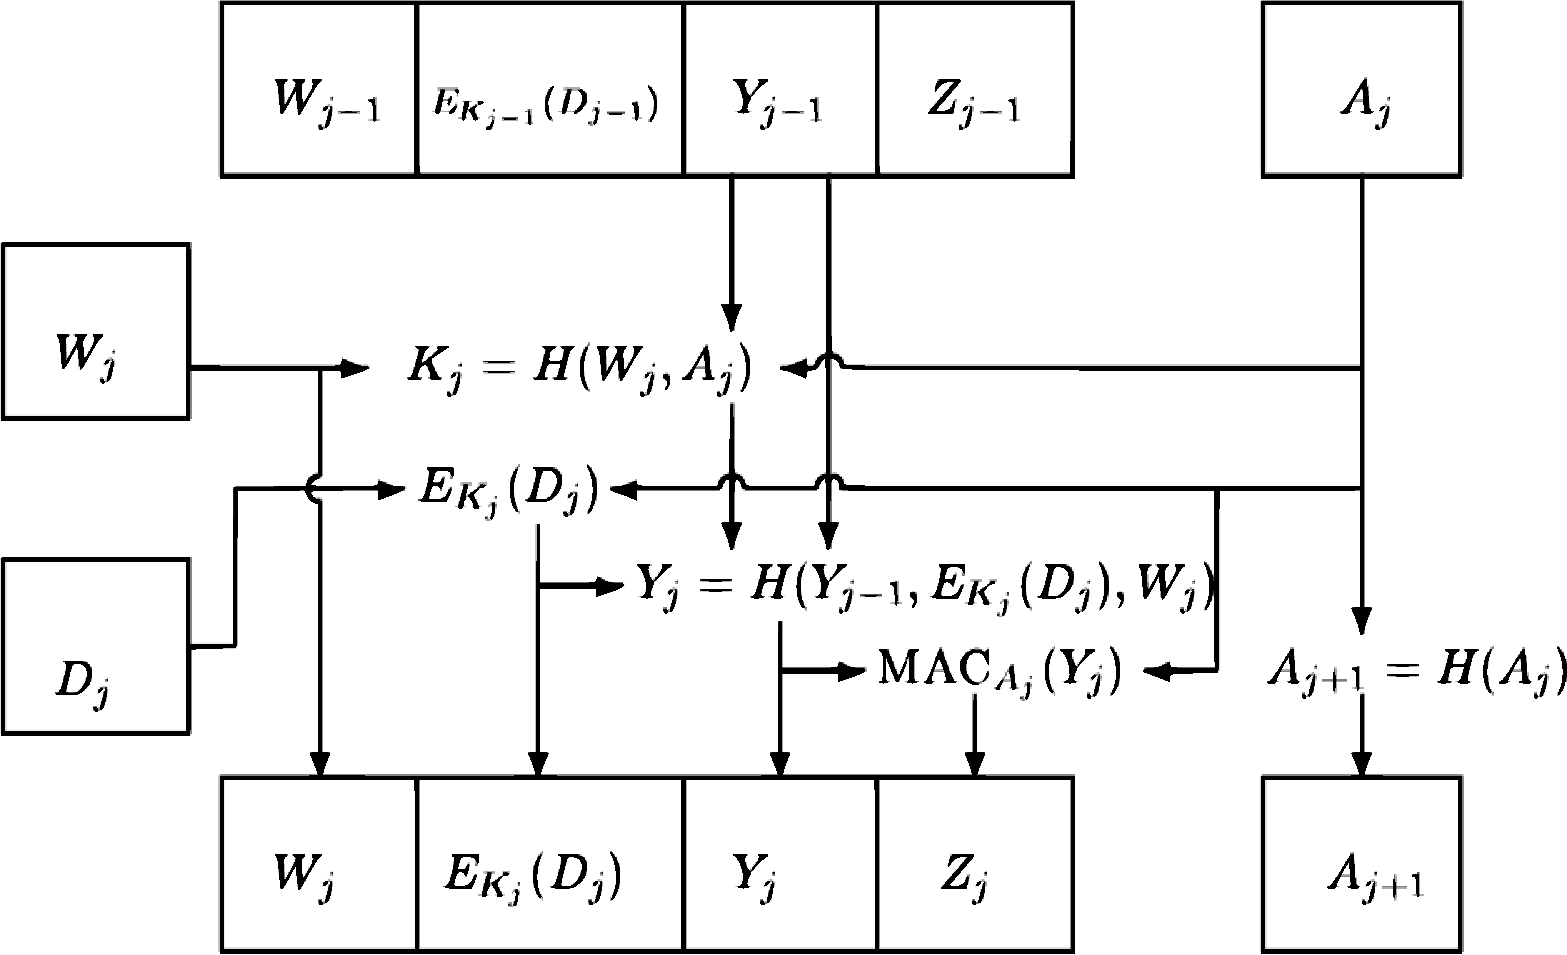
\includegraphics[scale=0.4]{images/sk-logentry-gen}
\caption{Schneier and Kelsey's log entry creation scheme.}
\label{fig:sk}
\end{center}
\end{figure}

%%%%%%%%%%%%%%%%%%%%%%%%%%%%%%%%%%%%%%%%%%%%%%%%%%%%%%%%%%%%%%%%%%%%%%%%
%%%%%%%%%%%%%%%%%%%%%%%%%%%%%%%%%%%%%%%%%%%%%%%%%%%%%%%%%%%%%%%%%%%%%%%%
%%%%%%%%%%%%%%%%%%%%%%%%%%%%%%%%%%%%%%%%%%%%%%%%%%%%%%%%%%%%%%%%%%%%%%%%

\section{Installation}

\libsklog allows to write applications which act as the actors \u, \t
and \v defined by Schneier and Kelsey. In this section is described
the \libsklog installation procedure and how to configure the
environment for each component of Scneier-Kelsey's schema.
All steps are described assuming that \libsklog installation
prefix is \texttt{/usr/local} and that a SQLite database is used to store
data locally.

%%%%%%%%%%%%%%%%%%%%%%%%%%%%%%%%%%%%%%%%%%%%%%%%%%%%%%%%%%%%%%%%%%%%%%%%
%%%%%%%%%%%%%%%%%%%%%%%%%%%%%%%%%%%%%%%%%%%%%%%%%%%%%%%%%%%%%%%%%%%%%%%%

\subsection{Get Sources and Install Library}

Before proceeding with the installation, the dependencies listed below
need to be resolved:

\begin{itemize}
\item \texttt{Libtool}
\item \texttt{Autoconf}
\item \texttt{OpenSSL $\ge$ 0.9.8}
\item \texttt{SQLite 3.x}
\item \texttt{libuuid-dev}
\item \texttt{libconfuse}
\end{itemize}

Installing \libsklog is rather painless through the use of the GNU
autoconf package. Simply get the sources from the Git\footnote{Git
Usage} repository, generate the \texttt{configure} script and
finally run it. In most cases, \texttt{configure} will automatically
determine everything it needs to know in order to compile. However,
there are a few options to ``configure'' to help it out, or change
the default behavior:
\ \\
\begin{lstlisting}
--enable-trace     Enable high verbosity mode for libsklog library
                   [default=no]

--enable-notify    Enable notify messages for libsklog library
                   [default=no]

--enable-debug     Enable debug support [default=no]
\end{lstlisting}
\ \\
The commands listed below, show you how to get the \libsklog sources,
how to generate the \texttt{configure} script and finally how to install
the library.
\ \\
%~ \lstset{caption=Get source code,captionpos=t}
\begin{lstlisting}
mkdir ~/temp
cd ~/temp
git clone https://github.com/psmiraglia/Libsklog.git libsklog

cd libsklog
mkdir m4
autoreconf --install --force --verbose

./configure --prefix=/usr/local [other options]
make
make install (as root)
\end{lstlisting}
\ \\
At this point the library should be correctly installed. Below is
reported the installation result. Now you can proceed with the
configuration of the components.
\ \\
%~ \lstset{caption=Result of the installation,captionpos=t}
\begin{lstlisting}
/usr/local
/usr/local/bin
/usr/local/bin/tnode
/usr/local/bin/unode
/usr/local/etc
/usr/local/etc/libsklog
/usr/local/etc/libsklog/certs
/usr/local/etc/libsklog/certs/ca
/usr/local/etc/libsklog/certs/ca/ca_cert.pem
/usr/local/etc/libsklog/certs/private
/usr/local/etc/libsklog/certs/private/ca_key.pem
/usr/local/etc/libsklog/certs/private/u1_key.pem
/usr/local/etc/libsklog/certs/u1_cert.pem
/usr/local/etc/libsklog/libsklog-t.conf.example
/usr/local/etc/libsklog/libsklog-u.conf.example
/usr/local/etc/libsklog/sql
/usr/local/etc/libsklog/sql/t_database.sql
/usr/local/etc/libsklog/sql/u_database.sql
/usr/local/include
/usr/local/include/libsklog
/usr/local/include/libsklog/sklog_commons.h
/usr/local/include/libsklog/sklog_err.h
/usr/local/include/libsklog/sklog_internal.h
/usr/local/include/libsklog/sklog_t.h
/usr/local/include/libsklog/sklog_u.h
/usr/local/include/libsklog/sklog_utils.h
/usr/local/include/libsklog/sklog_v.h
/usr/local/lib
/usr/local/lib/libsklog.a
/usr/local/lib/libsklog.la
/usr/local/lib/libsklog.so -> libsklog.so.0.0.0
/usr/local/lib/libsklog.so.0 -> libsklog.so.0.0.0
/usr/local/lib/libsklog.so.0.0.0
/usr/local/var
/usr/local/var/libsklog
/usr/local/var/libsklog/db
/usr/local/var/libsklog/db/t.db
/usr/local/var/libsklog/db/u.db
\end{lstlisting}


%%%%%%%%%%%%%%%%%%%%%%%%%%%%%%%%%%%%%%%%%%%%%%%%%%%%%%%%%%%%%%%%%%%%%%%%
%%%%%%%%%%%%%%%%%%%%%%%%%%%%%%%%%%%%%%%%%%%%%%%%%%%%%%%%%%%%%%%%%%%%%%%%

\subsection{Setup $\mathcal{U}$ Component}

\subsubsection{Configuration File}

To configure a \u component it's necessary to create a file called
\texttt{libsklog-u.conf} in \texttt{/usr/local/etc/libsklog} which
will contains all required settings. If the configuration file is
not present, default values will be used. Below all settable
parameters:

\begin{center}
\small{
\begin{tabular}{|p{.2\textwidth}|p{.7\textwidth}|}
\hline
\texttt{t\_cert} & Specifies the path where the certificate of \t is installed.
                   \t acts also as certification authority.\\ \hline
\texttt{t\_address} & Specifies the IP address of \t. \\ \hline
\texttt{t\_port} & Specifies the port on where \t is listening.\\ \hline
\texttt{u\_cert} & Specifies the path where the certificate of \u,
                   issued by \t, is installed. \\ \hline
\texttt{u\_id} & Specifies the identifier (common name) of \u.\\ \hline
\texttt{u\_privkey} & Specifies the path where the private key of \u is
                      installed. \\ \hline
\texttt{u\_timeout} & Sets the timeout for the logfile initialization
                      procedure.\\ \hline
\texttt{logfile\_size} & Sets the number of log entries which can be
                         collected into the logfile.\\ \hline
\end{tabular}
}
\end{center}

The file \texttt{libsklog-u.conf.example} is a template of a
configuration file for \u component. You can use it as staring point
for the definition of a new file:\ \\

\begin{lstlisting}
cd /usr/local/etc/libsklog
cp libsklog-u.conf.example libsklog-u.conf
vim libsklog-u.conf
(edit your file)
\end{lstlisting}

\subsubsection{Database Initialization}

\begin{lstlisting}
cd /usr/local/var/libsklog/db
sqlite3 u.db < /usr/local/etc/libsklog/sql/u_database.sql
\end{lstlisting}

%%%%%%%%%%%%%%%%%%%%%%%%%%%%%%%%%%%%%%%%%%%%%%%%%%%%%%%%%%%%%%%%%%%%%%%%
%%%%%%%%%%%%%%%%%%%%%%%%%%%%%%%%%%%%%%%%%%%%%%%%%%%%%%%%%%%%%%%%%%%%%%%%

\subsection{Setup $\mathcal{T}$ Component}

\subsubsection{Configuration File}

To configure a \t component it's necessary to create a file called
\texttt{libsklog-t.conf} in \texttt{/usr/local/etc/libsklog} which
will contains all required settings. If the configuration file is
not present, default values will be used. Below all settable
parameters:

\begin{center}
\small{
\begin{tabular}{|p{.2\textwidth}|p{.7\textwidth}|}
\hline
\texttt{t\_cert} & Specifies the path where the certificate of \t is installed.
                   \t acts also as certification authority.\\ \hline
\texttt{t\_privkey} & Specifies the path where the private key of \t is
                      installed. \\ \hline
\texttt{t\_id} & Specifies the identifier (common name) of \t.\\ \hline
\texttt{t\_address} & Specifies the IP address of \t. \\ \hline
\texttt{t\_port} & Specifies the port on where \t is listening.\\ \hline
\end{tabular}
}
\end{center}

The file \texttt{libsklog-t.conf.example} is a template of a
configuration file for \t component. You can use it as staring point
for the definition of a new file:\ \\

\begin{lstlisting}
cd /usr/local/etc/libsklog
cp libsklog-t.conf.example libsklog-t.conf
vim libsklog-t.conf
(edit your file)
\end{lstlisting}

\subsubsection{Database Initialization}

\begin{lstlisting}
cd /usr/local/var/libsklog/db
sqlite3 t.db < /usr/local/etc/libsklog/sql/t_database.sql
\end{lstlisting}


%%%%%%%%%%%%%%%%%%%%%%%%%%%%%%%%%%%%%%%%%%%%%%%%%%%%%%%%%%%%%%%%%%%%%%%%
%%%%%%%%%%%%%%%%%%%%%%%%%%%%%%%%%%%%%%%%%%%%%%%%%%%%%%%%%%%%%%%%%%%%%%%%

\subsection{Setup $\mathcal{V}$ Component}

Not yet implemented. Do you want to help me?

\newpage
\section{Usage}

The installation of libsklog provides two sample application called
\texttt{tnode} and \texttt{unode}. The applications are available
in the path \texttt{/usr/local/bin}. During the execution of the
application you have to provide a passphrase which is
"123456" if you use the default certificates.

\subsection{\u component}

\begin{lstlisting}
/*
** This is a really simple application
** which acts as U component
*/

#include <stdio.h>
#include <string.h>
#include <libsklog/sklog_u.h>

#define BUFLEN 1024

int main (void) {

    SKLOG_U_Ctx *ctx = 0;
    SKLOG_DATA_TYPE e_type = 0;
    char event[BUFLEN] = { 0 };

    ...

    ctx = SKLOG_U_NewCtx();

    if ( ctx == NULL ) {
        fprintf(stderr,"SKLOG_U_NewCtx() failure");
        exit(1);
    }

    /* something happens */
    SKLOG_U_LogEvent(ctx,e_type,event,strlen(event));

    ...

    /* something happens */
    SKLOG_U_LogEvent(ctx,e_type,event,strlen(event));

    ...

    /* something happens */
    SKLOG_U_LogEvent(ctx,e_type,event,strlen(event));

    ...

    SKLOG_U_FreeCtx(&ctx);

    return 0;
} 
\end{lstlisting}

\begin{lstlisting}
gcc -I/usr/local/include -L/usr/local/lib \
    u_app.c -o u_app -lsklog
\end{lstlisting}
\newpage
\subsection{\t component}
\begin{lstlisting}
/*
** This is a really simple application
** which acts as T component
*/

#include <stdio.h>
#include <libsklog/sklog_t.h>

#define BUFLEN 1024

int main (void) {

    SKLOG_T_Ctx *ctx = 0;

    ...

    ctx = SKLOG_T_NewCtx();

    if ( ctx == NULL ) {
        fprintf(stderr,"SKLOG_T_NewCtx() failure");
        exit(1);
    }

    if ( SKLOG_T_InitCtx(ctx) == SKLOG_FAILURE ) {
        fprintf(stderr,"SKLOG_T_InitCtx() failure");
        exit(1);
    }

    ...
    
    SKLOG_T_Run(ctx);

    ...

    SKLOG_T_FreeCtx(&ctx);

    return 0;
} 
\end{lstlisting}

\begin{lstlisting}
gcc -I/usr/local/include -L/usr/local/lib \
    t_app.c -o t_app -lsklog
\end{lstlisting}
\newpage
\section{TODO List}

\subsection{\u}

\begin{itemize}
\item Maybe nothing...
\end{itemize}

\subsection{\t}

\begin{itemize}
\item Implement function which parse the configuration file
\item Implement function which verify the M0 message
\item Implement function which verify the integrity of collected data
\end{itemize}

\subsection{\v}

\begin{itemize}
\item All! Do you want to help me?
\end{itemize}

\end{document}
